\section{Introduction}

	\subsection{Goal}
		The goal of this experiment is to determine the first excitation energy of mercury atoms in the vapor to come to the conclusion that atoms have discrete transition energies, thus confirming the quantum theory.
	
	\subsection{Theory}
		The Franck-Hertz experiment is one of the most significant experiments in history since it provided the first experimental conformation for the quantum nature of atoms, verifying the quantum theory with experimental data.
		\\
		\\
		The Bohr atom model states that electrons of atoms occupy certain discrete energy levels and that there are no intermediate levels. The experimental result showed that electrons can occupy higher energy levels if they absorb 4.9 eV of energy, directly verifying the Bohr atom model.
		\\
		\\
		Thermionic emission , which is the liberation of electrons with temperature, is used to eject electrons into the experimental apparatus which provides the energy necessary to excite the electrons in mercury gas. Electrons ejected by the cathode undergo collisions with mercury atoms in the gas. Electrons that have enough energy undergo inelastic collisions to excite the mercury electrons to higher states, resulting in a phase transition; on the other hand, electrons that does not have enough energy undergo elastic collisions and lose little to no energy which does not result in excitation.
		\\
		\\
		The heart of the underlying mechanism in this experiment can be investigated using the resulting current vs accelerating voltage data. When the electrons coming from the cathode elastically collide with the mercury atoms, they lose little to no energy and just change direction since the mercury atom is nearly four hundred thousand times more massive than the incident electrons. The same electrons can collide inelastically with the mercury atoms as their speeds exceed 1.3 million meters per second, which corresponds to a knietic energy of 4.9 electron volts. When the electrons collide inelastically, they transfer some of their energy to the mercury atoms to excite them, thus losing speed and kinetic energy; which results in the spikey behaviour present in the current vs accelerating voltage plot. We can draw a lot of conclusions from these current drops and they will all be carried out in the later sections of this report. A theoretical plot can be seen below.
		
		\begin{figure}[h!]
			\centering
			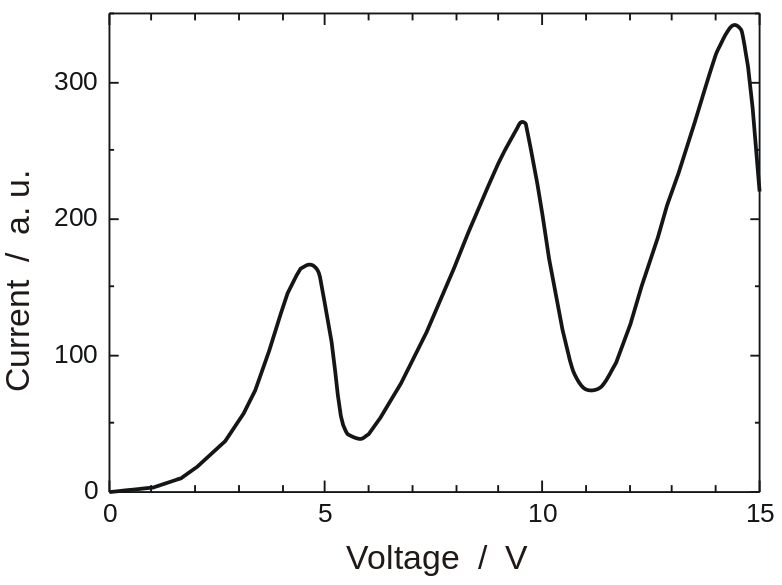
\includegraphics[width=0.5\textwidth]{images/fh_theo_plot.png}
			\label{fig: fh}
			\caption{Current vs Accelerating Voltage Plot}
		\end{figure}
		